
%% bare_jrnl_compsoc.tex
%% V1.4b
%% 2015/08/26
%% by Michael Shell
%% See:
%% http://www.michaelshell.org/
%% for current contact information.
%%
%% This is a skeleton file demonstrating the use of IEEEtran.cls
%% (requires IEEEtran.cls version 1.8b or later) with an IEEE
%% Computer Society journal paper.
%%
%% Support sites:
%% http://www.michaelshell.org/tex/ieeetran/
%% http://www.ctan.org/pkg/ieeetran
%% and
%% http://www.ieee.org/

%%*************************************************************************
%% Legal Notice:
%% This code is offered as-is without any warranty either expressed or
%% implied; without even the implied warranty of MERCHANTABILITY or
%% FITNESS FOR A PARTICULAR PURPOSE! 
%% User assumes all risk.
%% In no event shall the IEEE or any contributor to this code be liable for
%% any damages or losses, including, but not limited to, incidental,
%% consequential, or any other damages, resulting from the use or misuse
%% of any information contained here.
%%
%% All comments are the opinions of their respective authors and are not
%% necessarily endorsed by the IEEE.
%%
%% This work is distributed under the LaTeX Project Public License (LPPL)
%% ( http://www.latex-project.org/ ) version 1.3, and may be freely used,
%% distributed and modified. A copy of the LPPL, version 1.3, is included
%% in the base LaTeX documentation of all distributions of LaTeX released
%% 2003/12/01 or later.
%% Retain all contribution notices and credits.
%% ** Modified files should be clearly indicated as such, including  **
%% ** renaming them and changing author support contact information. **
%%*************************************************************************


% *** Authors should verify (and, if needed, correct) their LaTeX system  ***
% *** with the testflow diagnostic prior to trusting their LaTeX platform ***
% *** with production work. The IEEE's font choices and paper sizes can   ***
% *** trigger bugs that do not appear when using other class files.       ***                          ***
% The testflow support page is at:
% http://www.michaelshell.org/tex/testflow/


\documentclass[10pt,journal,compsoc]{IEEEtran}
%
% If IEEEtran.cls has not been installed into the LaTeX system files,
% manually specify the path to it like:
% \documentclass[10pt,journal,compsoc]{../sty/IEEEtran}





% Some very useful LaTeX packages include:
% (uncomment the ones you want to load)


% *** MISC UTILITY PACKAGES ***
%
%\usepackage{ifpdf}
% Heiko Oberdiek's ifpdf.sty is very useful if you need conditional
% compilation based on whether the output is pdf or dvi.
% usage:
% \ifpdf
%   % pdf code
% \else
%   % dvi code
% \fi
% The latest version of ifpdf.sty can be obtained from:
% http://www.ctan.org/pkg/ifpdf
% Also, note that IEEEtran.cls V1.7 and later provides a builtin
% \ifCLASSINFOpdf conditional that works the same way.
% When switching from latex to pdflatex and vice-versa, the compiler may
% have to be run twice to clear warning/error messages.






% *** CITATION PACKAGES ***
%
\ifCLASSOPTIONcompsoc
  % IEEE Computer Society needs nocompress option
  % requires cite.sty v4.0 or later (November 2003)
  \usepackage[nocompress]{cite}
\else
  % normal IEEE
  \usepackage{cite}
\fi
% cite.sty was written by Donald Arseneau
% V1.6 and later of IEEEtran pre-defines the format of the cite.sty package
% \cite{} output to follow that of the IEEE. Loading the cite package will
% result in citation numbers being automatically sorted and properly
% "compressed/ranged". e.g., [1], [9], [2], [7], [5], [6] without using
% cite.sty will become [1], [2], [5]--[7], [9] using cite.sty. cite.sty's
% \cite will automatically add leading space, if needed. Use cite.sty's
% noadjust option (cite.sty V3.8 and later) if you want to turn this off
% such as if a citation ever needs to be enclosed in parenthesis.
% cite.sty is already installed on most LaTeX systems. Be sure and use
% version 5.0 (2009-03-20) and later if using hyperref.sty.
% The latest version can be obtained at:
% http://www.ctan.org/pkg/cite
% The documentation is contained in the cite.sty file itself.
%
% Note that some packages require special options to format as the Computer
% Society requires. In particular, Computer Society  papers do not use
% compressed citation ranges as is done in typical IEEE papers
% (e.g., [1]-[4]). Instead, they list every citation separately in order
% (e.g., [1], [2], [3], [4]). To get the latter we need to load the cite
% package with the nocompress option which is supported by cite.sty v4.0
% and later. Note also the use of a CLASSOPTION conditional provided by
% IEEEtran.cls V1.7 and later.





% *** GRAPHICS RELATED PACKAGES ***
%
\ifCLASSINFOpdf
  \usepackage{graphicx}
  % declare the path(s) where your graphic files are
  \graphicspath{{Figures/}{Other_Folder/}}
  % and their extensions so you won't have to specify these with
  % every instance of \includegraphics
  \DeclareGraphicsExtensions{.pdf,.jpeg,.png}
\else
  % or other class option (dvipsone, dvipdf, if not using dvips). graphicx
  % will default to the driver specified in the system graphics.cfg if no
  % driver is specified.
  % \usepackage[dvips]{graphicx}
  % declare the path(s) where your graphic files are
  % \graphicspath{{../eps/}}
  % and their extensions so you won't have to specify these with
  % every instance of \includegraphics
  % \DeclareGraphicsExtensions{.eps}
\fi
% graphicx was written by David Carlisle and Sebastian Rahtz. It is
% required if you want graphics, photos, etc. graphicx.sty is already
% installed on most LaTeX systems. The latest version and documentation
% can be obtained at: 
% http://www.ctan.org/pkg/graphicx
% Another good source of documentation is "Using Imported Graphics in
% LaTeX2e" by Keith Reckdahl which can be found at:
% http://www.ctan.org/pkg/epslatex
%
% latex, and pdflatex in dvi mode, support graphics in encapsulated
% postscript (.eps) format. pdflatex in pdf mode supports graphics
% in .pdf, .jpeg, .png and .mps (metapost) formats. Users should ensure
% that all non-photo figures use a vector format (.eps, .pdf, .mps) and
% not a bitmapped formats (.jpeg, .png). The IEEE frowns on bitmapped formats
% which can result in "jaggedy"/blurry rendering of lines and letters as
% well as large increases in file sizes.
%
% You can find documentation about the pdfTeX application at:
% http://www.tug.org/applications/pdftex






% *** MATH PACKAGES ***
%
%\usepackage{amsmath}
% A popular package from the American Mathematical Society that provides
% many useful and powerful commands for dealing with mathematics.
%
% Note that the amsmath package sets \interdisplaylinepenalty to 10000
% thus preventing page breaks from occurring within multiline equations. Use:
%\interdisplaylinepenalty=2500
% after loading amsmath to restore such page breaks as IEEEtran.cls normally
% does. amsmath.sty is already installed on most LaTeX systems. The latest
% version and documentation can be obtained at:
% http://www.ctan.org/pkg/amsmath





% *** SPECIALIZED LIST PACKAGES ***
%
%\usepackage{algorithmic}
% algorithmic.sty was written by Peter Williams and Rogerio Brito.
% This package provides an algorithmic environment fo describing algorithms.
% You can use the algorithmic environment in-text or within a figure
% environment to provide for a floating algorithm. Do NOT use the algorithm
% floating environment provided by algorithm.sty (by the same authors) or
% algorithm2e.sty (by Christophe Fiorio) as the IEEE does not use dedicated
% algorithm float types and packages that provide these will not provide
% correct IEEE style captions. The latest version and documentation of
% algorithmic.sty can be obtained at:
% http://www.ctan.org/pkg/algorithms
% Also of interest may be the (relatively newer and more customizable)
% algorithmicx.sty package by Szasz Janos:
% http://www.ctan.org/pkg/algorithmicx




% *** ALIGNMENT PACKAGES ***
%
%\usepackage{array}
% Frank Mittelbach's and David Carlisle's array.sty patches and improves
% the standard LaTeX2e array and tabular environments to provide better
% appearance and additional user controls. As the default LaTeX2e table
% generation code is lacking to the point of almost being broken with
% respect to the quality of the end results, all users are strongly
% advised to use an enhanced (at the very least that provided by array.sty)
% set of table tools. array.sty is already installed on most systems. The
% latest version and documentation can be obtained at:
% http://www.ctan.org/pkg/array


% IEEEtran contains the IEEEeqnarray family of commands that can be used to
% generate multiline equations as well as matrices, tables, etc., of high
% quality.




% *** SUBFIGURE PACKAGES ***
\ifCLASSOPTIONcompsoc
 \usepackage[caption=false,font=footnotesize,labelfont=sf,textfont=sf]{subfig}
\else
 \usepackage[caption=false,font=footnotesize]{subfig}
\fi
% subfig.sty, written by Steven Douglas Cochran, is the modern replacement
% for subfigure.sty, the latter of which is no longer maintained and is
% incompatible with some LaTeX packages including fixltx2e. However,
% subfig.sty requires and automatically loads Axel Sommerfeldt's caption.sty
% which will override IEEEtran.cls' handling of captions and this will result
% in non-IEEE style figure/table captions. To prevent this problem, be sure
% and invoke subfig.sty's "caption=false" package option (available since
% subfig.sty version 1.3, 2005/06/28) as this is will preserve IEEEtran.cls
% handling of captions.
% Note that the Computer Society format requires a sans serif font rather
% than the serif font used in traditional IEEE formatting and thus the need
% to invoke different subfig.sty package options depending on whether
% compsoc mode has been enabled.
%
% The latest version and documentation of subfig.sty can be obtained at:
% http://www.ctan.org/pkg/subfig




% *** FLOAT PACKAGES ***
%
%\usepackage{fixltx2e}
% fixltx2e, the successor to the earlier fix2col.sty, was written by
% Frank Mittelbach and David Carlisle. This package corrects a few problems
% in the LaTeX2e kernel, the most notable of which is that in current
% LaTeX2e releases, the ordering of single and double column floats is not
% guaranteed to be preserved. Thus, an unpatched LaTeX2e can allow a
% single column figure to be placed prior to an earlier double column
% figure.
% Be aware that LaTeX2e kernels dated 2015 and later have fixltx2e.sty's
% corrections already built into the system in which case a warning will
% be issued if an attempt is made to load fixltx2e.sty as it is no longer
% needed.
% The latest version and documentation can be found at:
% http://www.ctan.org/pkg/fixltx2e


%\usepackage{stfloats}
% stfloats.sty was written by Sigitas Tolusis. This package gives LaTeX2e
% the ability to do double column floats at the bottom of the page as well
% as the top. (e.g., "\begin{figure*}[!b]" is not normally possible in
% LaTeX2e). It also provides a command:
%\fnbelowfloat
% to enable the placement of footnotes below bottom floats (the standard
% LaTeX2e kernel puts them above bottom floats). This is an invasive package
% which rewrites many portions of the LaTeX2e float routines. It may not work
% with other packages that modify the LaTeX2e float routines. The latest
% version and documentation can be obtained at:
% http://www.ctan.org/pkg/stfloats
% Do not use the stfloats baselinefloat ability as the IEEE does not allow
% \baselineskip to stretch. Authors submitting work to the IEEE should note
% that the IEEE rarely uses double column equations and that authors should try
% to avoid such use. Do not be tempted to use the cuted.sty or midfloat.sty
% packages (also by Sigitas Tolusis) as the IEEE does not format its papers in
% such ways.
% Do not attempt to use stfloats with fixltx2e as they are incompatible.
% Instead, use Morten Hogholm'a dblfloatfix which combines the features
% of both fixltx2e and stfloats:
%
% \usepackage{dblfloatfix}
% The latest version can be found at:
% http://www.ctan.org/pkg/dblfloatfix




%\ifCLASSOPTIONcaptionsoff
%  \usepackage[nomarkers]{endfloat}
% \let\MYoriglatexcaption\caption
% \renewcommand{\caption}[2][\relax]{\MYoriglatexcaption[#2]{#2}}
%\fi
% endfloat.sty was written by James Darrell McCauley, Jeff Goldberg and 
% Axel Sommerfeldt. This package may be useful when used in conjunction with 
% IEEEtran.cls'  captionsoff option. Some IEEE journals/societies require that
% submissions have lists of figures/tables at the end of the paper and that
% figures/tables without any captions are placed on a page by themselves at
% the end of the document. If needed, the draftcls IEEEtran class option or
% \CLASSINPUTbaselinestretch interface can be used to increase the line
% spacing as well. Be sure and use the nomarkers option of endfloat to
% prevent endfloat from "marking" where the figures would have been placed
% in the text. The two hack lines of code above are a slight modification of
% that suggested by in the endfloat docs (section 8.4.1) to ensure that
% the full captions always appear in the list of figures/tables - even if
% the user used the short optional argument of \caption[]{}.
% IEEE papers do not typically make use of \caption[]'s optional argument,
% so this should not be an issue. A similar trick can be used to disable
% captions of packages such as subfig.sty that lack options to turn off
% the subcaptions:
% For subfig.sty:
% \let\MYorigsubfloat\subfloat
% \renewcommand{\subfloat}[2][\relax]{\MYorigsubfloat[]{#2}}
% However, the above trick will not work if both optional arguments of
% the \subfloat command are used. Furthermore, there needs to be a
% description of each subfigure *somewhere* and endfloat does not add
% subfigure captions to its list of figures. Thus, the best approach is to
% avoid the use of subfigure captions (many IEEE journals avoid them anyway)
% and instead reference/explain all the subfigures within the main caption.
% The latest version of endfloat.sty and its documentation can obtained at:
% http://www.ctan.org/pkg/endfloat
%
% The IEEEtran \ifCLASSOPTIONcaptionsoff conditional can also be used
% later in the document, say, to conditionally put the References on a 
% page by themselves.




% *** PDF, URL AND HYPERLINK PACKAGES ***
%
\usepackage{url}
\usepackage{hyperref}
% url.sty was written by Donald Arseneau. It provides better support for
% handling and breaking URLs. url.sty is already installed on most LaTeX
% systems. The latest version and documentation can be obtained at:
% http://www.ctan.org/pkg/url
% Basically, \url{my_url_here}.





% *** Do not adjust lengths that control margins, column widths, etc. ***
% *** Do not use packages that alter fonts (such as pslatex).         ***
% There should be no need to do such things with IEEEtran.cls V1.6 and later.
% (Unless specifically asked to do so by the journal or conference you plan
% to submit to, of course. )


% correct bad hyphenation here
\hyphenation{op-tical net-works semi-conduc-tor}


\begin{document}
%
% paper title
% Titles are generally capitalized except for words such as a, an, and, as,
% at, but, by, for, in, nor, of, on, or, the, to and up, which are usually
% not capitalized unless they are the first or last word of the title.
% Linebreaks \\ can be used within to get better formatting as desired.
% Do not put math or special symbols in the title.
\title{Analysis on Time Improvements with Code Parallelization}
%
%
% author names and IEEE memberships
% note positions of commas and nonbreaking spaces ( ~ ) LaTeX will not break
% a structure at a ~ so this keeps an author's name from being broken across
% two lines.
% use \thanks{} to gain access to the first footnote area
% a separate \thanks must be used for each paragraph as LaTeX2e's \thanks
% was not built to handle multiple paragraphs
%
%
%\IEEEcompsocitemizethanks is a special \thanks that produces the bulleted
% lists the Computer Society journals use for "first footnote" author
% affiliations. Use \IEEEcompsocthanksitem which works much like \item
% for each affiliation group. When not in compsoc mode,
% \IEEEcompsocitemizethanks becomes like \thanks and
% \IEEEcompsocthanksitem becomes a line break with idention. This
% facilitates dual compilation, although admittedly the differences in the
% desired content of \author between the different types of papers makes a
% one-size-fits-all approach a daunting prospect. For instance, compsoc 
% journal papers have the author affiliations above the "Manuscript
% received ..."  text while in non-compsoc journals this is reversed. Sigh.

\author{Diogo~Rebimba,~\IEEEmembership{d.rebimba,~46731,}
        Hugo~Lopes,~\IEEEmembership{ha.lopes,~49873,}
        and~Diogo~Escaleira,~\IEEEmembership{d.escaleira,~50054}% <-this % stops a space
}
%\IEEEcompsocitemizethanks{\IEEEcompsocthanksitem M. Shell was with the Department
%of Electrical and Computer Engineering, Georgia Institute of Technology, Atlanta,
%GA, 30332.\protect\\
%% note need leading \protect in front of \\ to get a newline within \thanks as
%% \\ is fragile and will error, could use \hfil\break instead.
%E-mail: see http://www.michaelshell.org/contact.html
%\IEEEcompsocthanksitem J. Doe and J. Doe are with Anonymous University.}% <-this % stops an unwanted space
%\thanks{Manuscript received April 19, 2005; revised August 26, 2015.}}

% note the % following the last \IEEEmembership and also \thanks - 
% these prevent an unwanted space from occurring between the last author name
% and the end of the author line. i.e., if you had this:
% 
% \author{....lastname \thanks{...} \thanks{...} }
%                     ^------------^------------^----Do not want these spaces!
%
% a space would be appended to the last name and could cause every name on that
% line to be shifted left slightly. This is one of those "LaTeX things". For
% instance, "\textbf{A} \textbf{B}" will typeset as "A B" not "AB". To get
% "AB" then you have to do: "\textbf{A}\textbf{B}"
% \thanks is no different in this regard, so shield the last } of each \thanks
% that ends a line with a % and do not let a space in before the next \thanks.
% Spaces after \IEEEmembership other than the last one are OK (and needed) as
% you are supposed to have spaces between the names. For what it is worth,
% this is a minor point as most people would not even notice if the said evil
% space somehow managed to creep in.



% The paper headers
\markboth{Concurrency and Parallelism Course, June~2021}%
{Shell \MakeLowercase{\textit{et al.}}: Analysis on Time Improvements with Code Parallelization}
% The only time the second header will appear is for the odd numbered pages
% after the title page when using the twoside option.
% 
% *** Note that you probably will NOT want to include the author's ***
% *** name in the headers of peer review papers.                   ***
% You can use \ifCLASSOPTIONpeerreview for conditional compilation here if
% you desire.



% The publisher's ID mark at the bottom of the page is less important with
% Computer Society journal papers as those publications place the marks
% outside of the main text columns and, therefore, unlike regular IEEE
% journals, the available text space is not reduced by their presence.
% If you want to put a publisher's ID mark on the page you can do it like
% this:
%\IEEEpubid{0000--0000/00\$00.00~\copyright~2015 IEEE}
% or like this to get the Computer Society new two part style.
%\IEEEpubid{\makebox[\columnwidth]{\hfill 0000--0000/00/\$00.00~\copyright~2015 IEEE}%
%\hspace{\columnsep}\makebox[\columnwidth]{Published by the IEEE Computer Society\hfill}}
% Remember, if you use this you must call \IEEEpubidadjcol in the second
% column for its text to clear the IEEEpubid mark (Computer Society jorunal
% papers don't need this extra clearance.)



% use for special paper notices
%\IEEEspecialpapernotice{(Invited Paper)}



% for Computer Society papers, we must declare the abstract and index terms
% PRIOR to the title within the \IEEEtitleabstractindextext IEEEtran
% command as these need to go into the title area created by \maketitle.
% As a general rule, do not put math, special symbols or citations
% in the abstract or keywords.
\IEEEtitleabstractindextext{%
\begin{abstract}
Optimization through parallelization of the provided sequential code (based on the EduHPC’18 Peachy Assignment from the Trasgo Research Group of the Universidad de Valladolid). The goal was to improve the performance values via parallelization of code when dealing with large sets of data as well as analyse the results obtained. The parallelization was achieved through OpenMp. This work allows to conclude that the data to be processed may influence the parallelization strategy. Also, the data size is important in scaling the machines responsible to deal with said data.
\end{abstract}

% Note that keywords are not normally used for peerreview papers.
\begin{IEEEkeywords}
Computer Science, Parallel and Concurrent Computing, Time Optimization with Introduction of Concurrence
\end{IEEEkeywords}}


% make the title area
\maketitle


% To allow for easy dual compilation without having to reenter the
% abstract/keywords data, the \IEEEtitleabstractindextext text will
% not be used in maketitle, but will appear (i.e., to be "transported")
% here as \IEEEdisplaynontitleabstractindextext when the compsoc 
% or transmag modes are not selected <OR> if conference mode is selected 
% - because all conference papers position the abstract like regular
% papers do.
\IEEEdisplaynontitleabstractindextext
% \IEEEdisplaynontitleabstractindextext has no effect when using
% compsoc or transmag under a non-conference mode.



% For peer review papers, you can put extra information on the cover
% page as needed:
% \ifCLASSOPTIONpeerreview
% \begin{center} \bfseries EDICS Category: 3-BBND \end{center}
% \fi
%
% For peerreview papers, this IEEEtran command inserts a page break and
% creates the second title. It will be ignored for other modes.
\IEEEpeerreviewmaketitle



\IEEEraisesectionheading{\section{Introduction}\label{sec:introduction}}
% Computer Society journal (but not conference!) papers do something unusual
% with the very first section heading (almost always called "Introduction").
% They place it ABOVE the main text! IEEEtran.cls does not automatically do
% this for you, but you can achieve this effect with the provided
% \IEEEraisesectionheading{} command. Note the need to keep any \label that
% is to refer to the section immediately after \section in the above as
% \IEEEraisesectionheading puts \section within a raised box.




% The very first letter is a 2 line initial drop letter followed
% by the rest of the first word in caps (small caps for compsoc).
% 
% form to use if the first word consists of a single letter:
% \IEEEPARstart{A}{demo} file is ....
% 
% form to use if you need the single drop letter followed by
% normal text (unknown if ever used by the IEEE):
% \IEEEPARstart{A}{}demo file is ....
% 
% Some journals put the first two words in caps:
% \IEEEPARstart{T}{his demo} file is ....
% 
% Here we have the typical use of a "T" for an initial drop letter
% and "HIS" in caps to complete the first word.
\IEEEPARstart{T}{his} report concerns a project for the course of Concurrency and Parallelism consists in the parallelization of a provided sequential program that simulates the effects of high-energy particles bombardment on an exposed surface, using the OpenMP programming model.\\
The program receives as input several files that represent waves of high-energy particles. It then computes the accumulated energy on each point of the surface after the impact of those waves. The program calculates and reports, for each wave, the point with the highest accumulated energy, which presents the higher risk of being damaged.\\
The main goal of this assignment is to improve the time performance of the source code, in particular when handling large sets of data (big number of particles). The challenge was, not only to find a way to parallelize the various sections of the sequential program, but also to analyse whether the achieved parallelizations are in fact worth it.
Our approach focused mainly on the identification and removal of dependencies in the various loops present in the source code, followed by parallelization using OpenMP and analysis of the possible performance improvements.


%\hfill mds
 
\hfill June 6, 2021

%\subsection{Subsection Heading Here}
%Subsection text here.

% needed in second column of first page if using \IEEEpubid
%\IEEEpubidadjcol

%\subsubsection{Subsubsection Heading Here}
%Subsubsection text here.


% An example of a floating figure using the graphicx package.
% Note that \label must occur AFTER (or within) \caption.
% For figures, \caption should occur after the \includegraphics.
% Note that IEEEtran v1.7 and later has special internal code that
% is designed to preserve the operation of \label within \caption
% even when the captionsoff option is in effect. However, because
% of issues like this, it may be the safest practice to put all your
% \label just after \caption rather than within \caption{}.
%
% Reminder: the "draftcls" or "draftclsnofoot", not "draft", class
% option should be used if it is desired that the figures are to be
% displayed while in draft mode.
%
%\begin{figure}[!t]
%\centering
%\includegraphics[width=2.5in]{myfigure}
% where an .eps filename suffix will be assumed under latex, 
% and a .pdf suffix will be assumed for pdflatex; or what has been declared
% via \DeclareGraphicsExtensions.
%\caption{Simulation results for the network.}
%\label{fig_sim}
%\end{figure}

% Note that the IEEE typically puts floats only at the top, even when this
% results in a large percentage of a column being occupied by floats.
% However, the Computer Society has been known to put floats at the bottom.


% An example of a double column floating figure using two subfigures.
% (The subfig.sty package must be loaded for this to work.)
% The subfigure \label commands are set within each subfloat command,
% and the \label for the overall figure must come after \caption.
% \hfil is used as a separator to get equal spacing.
% Watch out that the combined width of all the subfigures on a 
% line do not exceed the text width or a line break will occur.
%
%\begin{figure*}[!t]
%\centering
%\subfloat[Case I]{\includegraphics[width=2.5in]{box}%
%\label{fig_first_case}}
%\hfil
%\subfloat[Case II]{\includegraphics[width=2.5in]{box}%
%\label{fig_second_case}}
%\caption{Simulation results for the network.}
%\label{fig_sim}
%\end{figure*}
%
% Note that often IEEE papers with subfigures do not employ subfigure
% captions (using the optional argument to \subfloat[]), but instead will
% reference/describe all of them (a), (b), etc., within the main caption.
% Be aware that for subfig.sty to generate the (a), (b), etc., subfigure
% labels, the optional argument to \subfloat must be present. If a
% subcaption is not desired, just leave its contents blank,
% e.g., \subfloat[].


% An example of a floating table. Note that, for IEEE style tables, the
% \caption command should come BEFORE the table and, given that table
% captions serve much like titles, are usually capitalized except for words
% such as a, an, and, as, at, but, by, for, in, nor, of, on, or, the, to
% and up, which are usually not capitalized unless they are the first or
% last word of the caption. Table text will default to \footnotesize as
% the IEEE normally uses this smaller font for tables.
% The \label must come after \caption as always.
%
%\begin{table}[!t]
%% increase table row spacing, adjust to taste
%\renewcommand{\arraystretch}{1.3}
% if using array.sty, it might be a good idea to tweak the value of
% \extrarowheight as needed to properly center the text within the cells
%\caption{An Example of a Table}
%\label{table_example}
%\centering
%% Some packages, such as MDW tools, offer better commands for making tables
%% than the plain LaTeX2e tabular which is used here.
%\begin{tabular}{|c||c|}
%\hline
%One & Two\\
%\hline
%Three & Four\\
%\hline
%\end{tabular}
%\end{table}


% Note that the IEEE does not put floats in the very first column
% - or typically anywhere on the first page for that matter. Also,
% in-text middle ("here") positioning is typically not used, but it
% is allowed and encouraged for Computer Society conferences (but
% not Computer Society journals). Most IEEE journals/conferences use
% top floats exclusively. 
% Note that, LaTeX2e, unlike IEEE journals/conferences, places
% footnotes above bottom floats. This can be corrected via the
% \fnbelowfloat command of the stfloats package.
\section{Development Methodology}
The following strategy was defined for the development of the work assignment: identify all loop dependencies; check the possibility of merges between loops; in the loops that have removable dependencies, remove them in order to parallelize the loops; use a profiler to check which methods have the most calls and how that affects the performance of the program. 
\\
During the development and analysis stage, this process had to be repeated to check if everything remains correctly parallelized after all the changes.

\subsection{ Dependency Analysis and Code Improvements }

%\paragraph*{}
\subsubsection{}
As previously stated, we started by identifying all the for loops dependencies. This way we could check whether each loop could be directly parallelized (using omp parallel for). In this first step, we found that:
\begin{itemize}
\item the loops in 4.2 (4.2.1 and 4.2.2) and 4.1.1 (the one with the update function) did not have dependencies. So, they could be directly parallelized.
\item the loop 4.3 had an output-dependency and flow-dependency.
\item the loop 4 has all the three dependencies (flow, output and anti).
\item The loop 4.1 has an output-dependency.
\end{itemize}

%\paragraph*{}
\subsubsection{}
We then tried to look for loops with the same parameters to check the possibility of a merger. In this step, we chose the 4.3 and 4.2.2 for loops: we tried several approaches, but ended up concluding that this merge is impossible due to a flow-dependency and anti-dependency, detected after merging the loops:
layer[k] $=$ … and if (layer[k] $>$ layer[k - 1] \&\& layer[k] $>$ layer[k + 1]) → anti dependency in k+1, flow dependency in k-1
(line 256)
As such, we returned the code to its previous form.

%\paragraph*{}
\subsubsection{}
As previously acknowledged, we detected an output-dependency on the 4.3 loop for. This dependency was resolved by splitting the loop in two: a parallelizable one, that uses two auxiliary arrays and the number of the thread to calculate local thread maximums, and the second one that compares the thread maximums to find the storm maximum and its position. With this change, we were able to improve the overall performance.

%\paragraph*{}
\subsubsection{}
In the last step of our strategy, we used a profiler: we experimented with multiple profiling tools (like Valgrind with the Callgrind tool as well as the CLion IDE profiling tool) and maintained the same conclusions. In figure \ref{profiler-pic}, obtained by using Kcachegrind visualizer for the Valgrind-Callgrind profiler using the sequential version of the program, we obtained an understanding of which methods have the most impact on the performance of our program. With this tool we can check the entire call tree which let us know which methods consume longer processing times. The majority of the calls were to the update method and the remaining were calls to procedures concerning the reading of the files which wasn't accounted for the times obtained. 
Another point we noticed from the other profiler tool (CLion IDE profiling tool) was that one of the methods that had more samples (meaning, the one that was most "called"), together with the update method, were the processes concerning the calls to omp parallel. From this information we can determine that some operations are not worth parallelizing because the gains from achieved through parallelizing such operations are surpassed by the costs of the procedures concerning the parallelization itself (like opening and closing threads).

\begin{figure}[h]
\centering
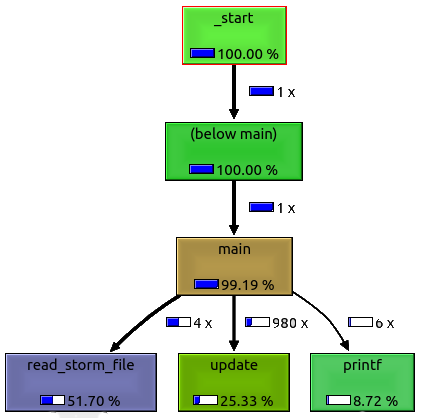
\includegraphics[scale=0.5]{../../profile_Valgrind.png}
\caption{Output of Valgrind profiler for sequential version}
\label{profiler-pic}
\end{figure}

\section{Testing and Results}

Before running the tests in the cluster in order to get results to withdraw conclusions, we run the tests in a day-to-day use Linux machine. In this pre-tests we realise that the average standard deviation in 5 runs is very low ($<$ 0.09). Furthermore, the environment on the cluster machine is much more controlled and free of interferences (regarding timing operations) so, in order to be able to execute more tests and since the time available on the cluster was limited, we decided to run each test only 2 times. 
\\
The used cluster machine has 4 x 8 processors and 32 hardware-threads. The tests were executed using a variable amount of threads from 1 (corresponding to sequential execution) to 32.
\\
All the executions of the parallelized code have proven to be accurate in terms of output compared with the unchanged sequential version. So the results never changed, only the execution time. Once the main purpose of this course is the study of concurrency and it's performance advantages, the results of the executions will not be presented although they were used to check the referred accuracy.

\subsection{Tests and Expectations}
\paragraph*{\textbf{Test 0}}
Using a test file provided by another group which we duly acknowledge, the execution of this test purpose is debugging and not performance analysis. For this reason it is not executed and timed in the test batch.

\paragraph*{\textbf{Test 1}}
The most basic and smallest test, mainly used for reference timing and debugging.
\\
Due to the small size, the anticipated results in terms of performance are not good since the times are so low they may not be worth the cost of thread opening.

\paragraph*{\textbf{Test 2}}
This is a small workload test where we expect some gains on small amount of thread opening. The increase in the number of threads would cause too much of an overhead cost (due to creation and management) that may not be softened by the increased processing speed.

\paragraph*{\textbf{Test 3 to 5}}
This group of tests are presented for completeness once their main goal was to find errors in race conditions. As suggested by the professor who provided the tests, they were executed only for at most 4 threads so it was decided to execute them just in our local machine.  
\\
Due to their very small size,the workload for each thread would be very small and it probably will not make up for the thread management costs.

\paragraph*{\textbf{Test 6}}
Originally this test was just like tests 3 to 5. We then decided to make some changes. It still uses small size wave arrays (however, bigger then the previous ones) but the main difference is that there are a considerable amount of waves.
\\
This test is expected to be the worst in performance given that all the optimizations made are in the calculations executed in each wave. This causes threads to be created several times to perform very small workloads.

\paragraph*{\textbf{Test 7}}
Decent size test. The main goal with it is to find if the optimizations done actually produced some effect on performance. It can be seen as the most balanced and close to reality test.\\
Before running predictions are that the increase of the thread number will produce speed-ups and, therefore, performance gains.

\paragraph*{\textbf{Test 8}}
Used to test the reduction efficiency of the solution, this test uses very big arrays (a lot of possible positions to be hit in each wave) but only one point (particle) per wave.
\\
Since the solution goes goes through the entire array, it's expected that the execution uses as much time as if it had a lot of points. And consequently of the same time pattern, similar speed-ups.

\paragraph*{\textbf{Test 9}}
We used this test either with 16 and 17 array positions as instructed. Since this test, like test 0, is focused on checking results and finding bugs in our development, it was decided not to run it in the cluster machine to make performance evaluations.

\paragraph*{\textbf{Test 10}}
This big size test was knowingly created to provide the perfect conditions for speed-ups according to the changes made in the parallel version. It uses a big array with several points but in single wave.
\\
Since there is a single file with a lot of points, it should be possible to see speed-ups every time the number of threads increases.

\paragraph*{\textbf{Test 11}}
This is the exact same test as \textit{test 10} but with the wave file used twice in order to create two waves. The goal is to check how the performance degrades with the number of waves by comparing these results with the previous ones.
\\
We expect the the drop in performance to be linear as the number of waves increases.

\subsection{Results}
In table \ref{aetC-tab} (displayed below) are the results of test execution on cluster. These are the main focus of the analysis being made in the work. 
\\
The results obtained are consistent with those which were expected.  Except for test 2 where the workload was expected to be too small to present improvements in every thread number increase but it ends up to be big enough to show some improvements.
\\
The times of test 11 are approximately the double of the ones on test 10. This shows that, although the prediction that test 11 was going to be worst than the 10 one, it gets worst in a linear way with the number of wave files considering the files are all the same size.
\\
An interesting and unexpected result is the similarity between the test 7 and 11. As exposed in the previous section, these two tests are totally unrelated and neither the number of points per wave neither the number of files are the same. The only similarity is that the array size is the same. It looked acceptable to extrapolate that the size of the array is not the main cause of variance in time of execution, instead, it's probably an equilibrium point where the bigger amount of smaller files in 7 increases the time cost by the amount of threads created for small workloads and the bigger and less amount of files in 11 have less thread management costs but more work to be done for each one of them.
\\
\begin{table}[h]
\centering
\caption{Output of Valgrind profiler for sequential version}
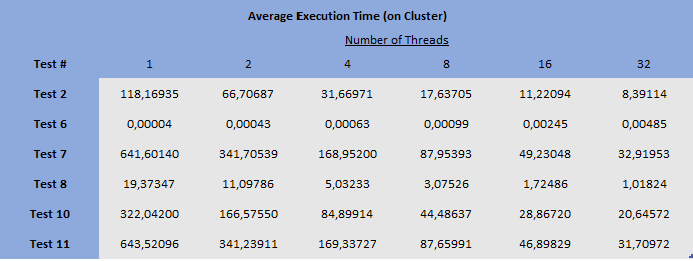
\includegraphics[width=0.5\textwidth]{../DRAFT/PerformanceAnalysis - Prints/Average Execution Time (cluster) - Table.PNG} 
\label{aetC-tab}
\end{table}
\\
Below it's presented in table \ref{aetL-tab} the results of the tests which were run in the local machine. Like it's mentioned earlier, these are mostly presented for completeness. As registered in the cluster for test 6, all the tests chosen to be run locally see their execution times worsen as the number of threads increases because this tests’ main purpose is not to evaluate the performance of the program but debugging and testing its correctness. Since the data to be computed is relatively small the parallelization costs outweigh the parallelization gains. 
\begin{table}[h]
\centering
\caption{Output of Valgrind profiler for sequential version}
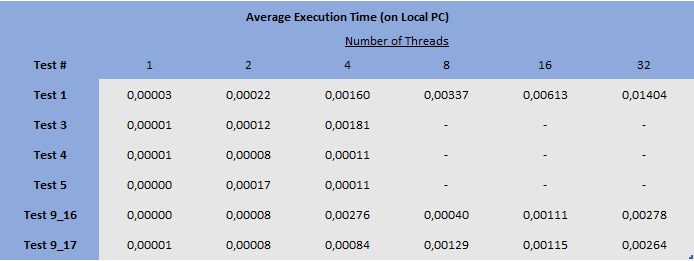
\includegraphics[width=0.5\textwidth]{../DRAFT/PerformanceAnalysis - Prints/Average Execution Time (local) - Table.PNG}
\label{aetL-tab}
\end{table}

\section{Analysis}
With the time values registered from the tests, presented in table \ref{aetC-tab}, it's possible to generate the graphics presented next. These graphics allow a better visualization of the results and consequently an easier way to conduct an analysis.
\\
All tests see their execution times reduced significantly as the number of threads increases. The exception is the test 6. Beware that, while the graph \ref{timeEv-pic} is helpful to understand the time evolution among the thread numbers, it doesn't fully reveal how badly the increase of the thread's number makes the execution time of test 6 increase. Also, due to the similarity of time values for the test 7 and 11 the lines overlap.  
\begin{figure}[h]
\centering
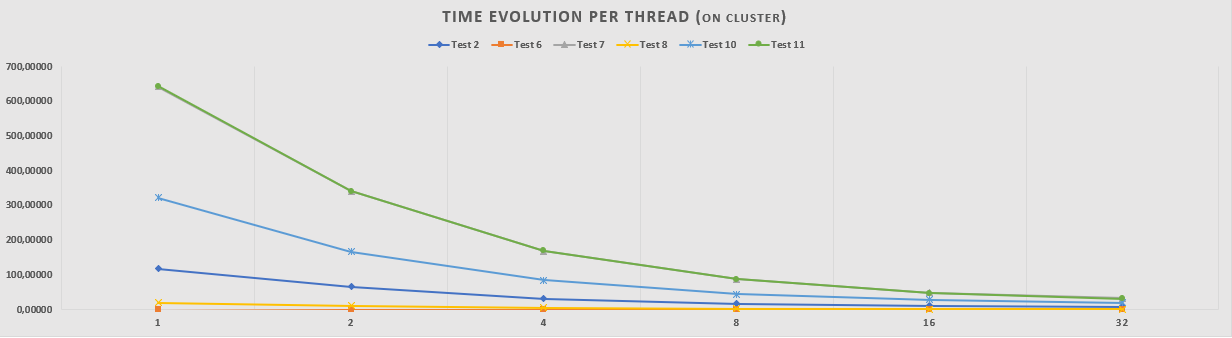
\includegraphics[width=0.5\textwidth]{../DRAFT/PerformanceAnalysis - Prints/Time Evolution per thread (cluster) - Chart.PNG}
\caption{Evolution of execution time for test per number of threads}
\label{timeEv-pic}
\end{figure}
\\
\\
The speed-up \textit{Sp} given by the formula presented below where \textit{T1} is the time of the sequential execution and \textit{Tp} the time of the parallel version with \textit{p} threads, the following graph was built.
\[ Sp = \frac{T1}{Tp} \]

\begin{figure}[h]
\centering
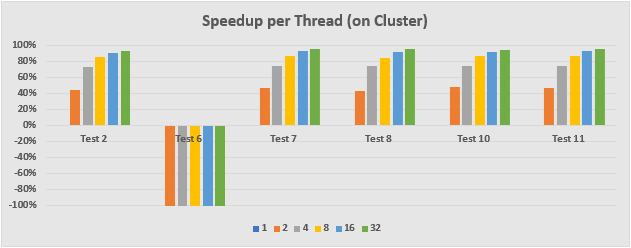
\includegraphics[width=0.5\textwidth]{../DRAFT/PerformanceAnalysis - Prints/Speedup per Thread (cluster) - Chart.PNG}
\caption{Speed-up achieved with each number of threads pre test}
\label{Sup-pic}
\end{figure}
As illustrated below in image \ref{Sup-pic}, all tests (except test 6) achieved great improvements, especially when increasing the number of threads from 1 to 2 (40-50\%) and from 2 to 4 (20-30\%). After that, as the number of threads increases, the speed-up gains become progressively less pronounced.
\\
In test 6 the speed-ups are really bad as predicted. They actually achieve values of around -10000\% not presented on the graph for visual purposes. This is caused by a large number of thread management operations (creation and join/destruction) related to the number of files used as well as a small workload to be carried out by each one of them. This occurs because the paralellisation strategy was focused on the most time consuming methods (update) and the wave/file computation wasn't made parallel.
\\
Once the speed-up for each test-number of threads pair was calculated, it's possible to use that to estimate the efficiency \textit{Ep} according to the number of threads \textit{p}

\[ Ep = \frac{Sp}{p} \]

\begin{table}[h]
\centering
\caption{Computation efficiency accordingly to the number of threads}
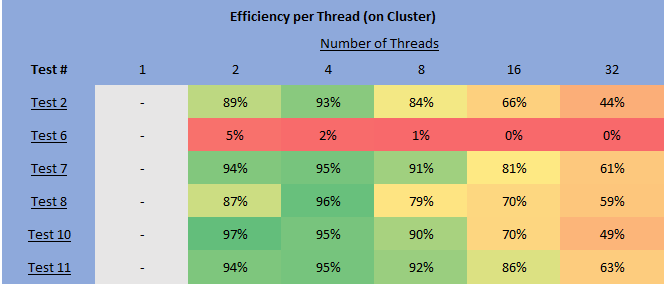
\includegraphics[width=0.5\textwidth]{../DRAFT/PerformanceAnalysis - Prints/Efficiency per Thread (cluster) - Chart.PNG}
\label{effic-table}
\end{table}

It's clear that great efficiency values are achieved with 2 and 4 threads, the latter's being the best values of the whole batch. Besides that, increasing the number of threads further than 8 is quite inefficient as the speed-up gains do not measure up.
\\
As expected and mentioned earlier, the test 6 presents very bad results.

\section{Conclusion}
Based on the analysis presented before, it can be concluded that it's not always a good approach to parallelize a sequential program. 
\\
The purpose of the computation as well as the kind of data to be used are two important aspects to take in consideration when parallelizing a program. The tests carried out show that the strategy used in this work is adequate to very large files but in small amounts. If the number of files increased while their size decreased a different approach would have to be taken or else it would be better to use the sequential version.
\\
Also, the availability of powerful machines with lots of processors isn't always good. In this case with the type of data used, never seems to be profitable to use more then 8 threads given that the efficiency will only degrade and the speed-ups achieved are not that significant.





% if have a single appendix:
%\appendix[Proof of the Zonklar Equations]
% or
%\appendix  % for no appendix heading
% do not use \section anymore after \appendix, only \section*
% is possibly needed

% use appendices with more than one appendix
% then use \section to start each appendix
% you must declare a \section before using any
% \subsection or using \label (\appendices by itself
% starts a section numbered zero.)
%


%\appendices

%\pagebreak

%\section{Extra}
%Evaluation part

% Can use something like this to put references on a page
% by themselves when using endfloat and the captionsoff option.
\ifCLASSOPTIONcaptionsoff
  \newpage
\fi



% trigger a \newpage just before the given reference
% number - used to balance the columns on the last page
% adjust value as needed - may need to be readjusted if
% the document is modified later
%\IEEEtriggeratref{8}
% The "triggered" command can be changed if desired:
%\IEEEtriggercmd{\enlargethispage{-5in}}

% references section

% can use a bibliography generated by BibTeX as a .bbl file
% BibTeX documentation can be easily obtained at:
% http://mirror.ctan.org/biblio/bibtex/contrib/doc/
% The IEEEtran BibTeX style support page is at:
% http://www.michaelshell.org/tex/ieeetran/bibtex/
%\bibliographystyle{IEEEtran}
% argument is your BibTeX string definitions and bibliography database(s)
%\bibliography{IEEEabrv,../bib/paper}
%
% <OR> manually copy in the resultant .bbl file
% set second argument of \begin to the number of references
% (used to reserve space for the reference number labels box)
%Para referenciar:\\
%- $https://pt.overleaf.com/learn/latex/Inserting_Images$

\begin{thebibliography}{1}

\bibitem{omp}
R. Rocha, “Programação em Memória Paralela com o OpenMP,” 2009. [Online]. Available: https://www.dcc.fc.up.pt/~ricroc/aulas/0910/ppd/apontamentos/openmp.pdf

\bibitem{deps}
J. Lourenço, “Parallel Programming Models and Dependences,” 2021

\end{thebibliography}


% use section* for acknowledgment
\ifCLASSOPTIONcompsoc
  % The Computer Society usually uses the plural form
  \section*{Acknowledgments}
\else
  % regular IEEE prefers the singular form
  \section*{Acknowledgment}
\fi


The authors would like to thank...
\begin{itemize}
\item Rúben Barreiro (42648) for asking a question on piazza which talked about a profiler that we later use
\\
\item David Pereira (52890) and his group (G28) for the python script base to generate test files
\\
\item The group who shared the \textit{layer35\_maximums\_0} test file (not properly identified in the piazza post) for the test file which helped us find bugs and dependencies. 
\end{itemize}

\section*{Individual Contribution}
\subsection*{Diogo Rebimba - 25\%}
\begin{itemize}
\item Parallel testing and analysis of loop 4.1 and merge of 4.3 with 4.2.2.
\item Profiler results analysis
\item Data treatment from test results
\item Excel graphs production for better visualization
\item Report production
\end{itemize}

\subsection*{Hugo Lopes - 50\%}
\begin{itemize}
\item Team management
\item Analysis and paralelization of loops 4.1, 4.2.1 and 4.2.2
\item Creation of test scripts
\item Cluster test and use
\item Report production and merge
\end{itemize}

\subsection*{Diogo Escaleira - 25\%}
\begin{itemize}
\item Parallelization, testing and analysis of loops 4, 4.1 and 4.3
\item Report production
\end{itemize}

\section*{comments, critics, and suggestions}
The size of the work seemed adequate to the time given as well as the difficult seemed appropriate.
We wish we could have had a bit more time in the DI Cluster but we do understand the the limitations imposed.
% that's all folks
\end{document}


